\documentclass[main]{subfiles}


\begin{document}
\newpage
\section{Continual-, Meta- And Transfer-Learning}

\subsection{Motivation}
In \cref{sec:challenges} we listed the standing challenges in deep learning research, from which we now want to discuss continual learning (the capability to learn multiple tasks sequentially) and meta-learning, which can allow to learn fast and from few-data only. So why do we need continual and meta-learning?
\begin{itemize}
    \item For many applications we don’t have large training data-sets (medical imaging, robotics, recommendations, real-world agent training).
    \item Life-long learning systems should quickly adapt to new tasks, but not forget previous ones (can’t learn every task/classifier from scratch).
    \item Sometimes our training data has a long-tail, meaning that there are only a few data points for a large range of categories.
    \item Concept learning enables humans to extrapolate from learned tasks to a similar task.
\end{itemize}

\begin{figure}[H]
    \centering
    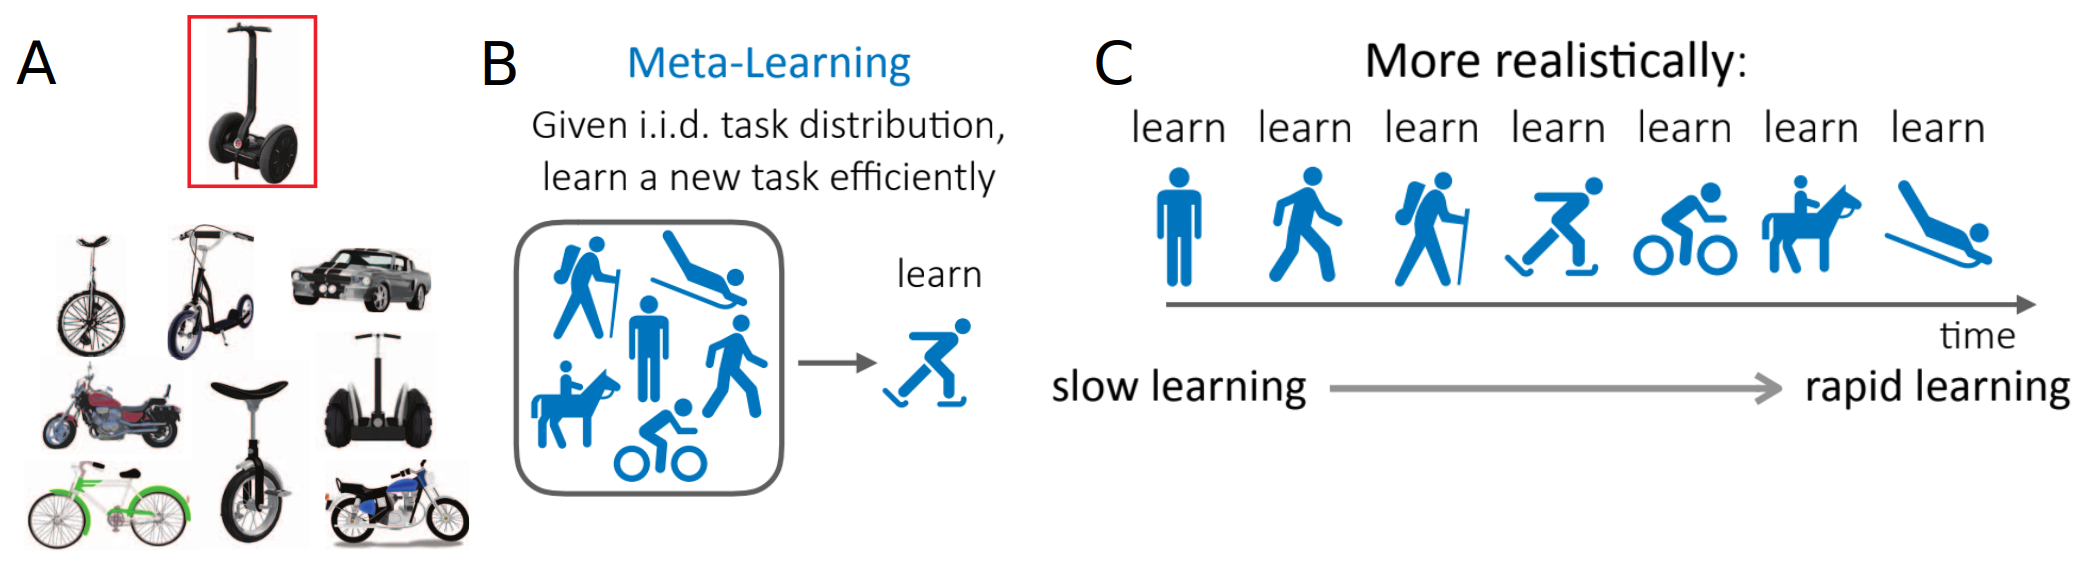
\includegraphics[width=0.99\linewidth]{14_ContinualMetaAndTransferLearning/figures/metalearning.png}
    \caption{The principle of learning the learn.}
    \label{fig:my_label}
\end{figure}

\subsection{Meta-Learning with ANNs}
Meta-learning, also known as “learning to learn”, intends to design models that can learn new skills or adapt to new environments rapidly with a few training examples. There are three common approaches\footnote{Awesome blog post by Lilian at OpenAI, where apparently half of the lecture was taken from: \url{https://lilianweng.github.io/lil-log/2018/11/30/meta-learning.html}}: 
\begin{enumerate}
    \item learn an efficient distance metric (metric-based)
    \item use (recurrent) network with external or internal memory (model-based)
    \item optimize the model parameters explicitly for fast learning (optimization-based)
\end{enumerate}

A good meta-learning model should be trained over a variety of learning tasks and optimized for the best performance on a distribution of tasks, including potentially unseen tasks. Each task is associated with a dataset $\mathcal{D}$, containing both feature vectors and true labels. The optimal model parameters are:
%
\begin{equation}
\theta^{*}=\arg \min _{\theta} \mathbb{E}_{\mathcal{D} \sim p(\mathcal{D})}\left[\mathcal{L}_{\theta}(\mathcal{D})\right]
\end{equation}
%
It looks very similar to a normal learning task, but one \textit{dataset} is considered as one \textit{data sample}. The concept of \textit{Few-shot classification} is an instantiation of meta-learning in the field of supervised learning. The dataset $\mathcal{D}$ is often split into two parts, a support set $\mathcal{S}$ for learning and a prediction set $\mathcal{B}$ for training or testing,  $\mathcal{D}=\langle S, B\rangle$. 

Another popular view of meta-learning decomposes the model update into two stages:
\begin{enumerate}
    \item A classifier $f_{\theta}$ is the "learner" model, trained for operating a given task
    \item In the meantime, a optimizer $g_{\phi}$ (the "meta-learner"), learns how to update the learner model's parameters via the support set $S, \theta^{'} = g_{\phi}(\theta, S).$
\end{enumerate}
In the final optimization step, one needs to update both $\theta$ and $\phi$ to maximize:
\begin{equation}
\mathbb{E}_{L \subset \mathcal{L}}\left[\mathbb{E}_{S^{L}} \subset \mathcal{D}, B^{L} \subset \mathcal{D}\left[\sum_{(\mathbf{x}, y) \in B^{L}} P_{g_{\phi}\left(\theta, S^{L}\right)}(y | \mathbf{x})\right]\right]
\end{equation}



\subsubsection{Metric-based ML}
The core idea in metric-based meta-learning is similar to nearest neighbors algorithms and kernel density estimation. The predicted probability over a set of known labels $y$ is a weighted sum of labels of support set samples. The weight is generated by a kernel function $k_\theta$, measuring the similarity between two data samples.
%
\begin{equation}
P_{\theta}(y | \mathbf{x}, S)=\sum_{\left(x_{i}, y_{i}\right) \in S} k_{\theta}\left(\mathbf{x}, \mathbf{x}_{i}\right) y_{i}
\end{equation}
%
To learn a good kernel is crucial to the success of a metric-based meta-learning model. Metric learning is well aligned with this intention, as it aims to learn a metric or distance function over objects. The notion of a good metric is problem-dependent. It should represent the relationship between inputs in the task space and facilitate problem solving. A few models are introduced, that learn embedding vectors of input data explicitly and use them to design proper kernel functions:

\paragraph{Prototypical Networks}\footnote{Snell\&Swersky\& Zemel, "Prototypical Networks for Few-shot Learning", 2017} use an embedding function $f_\theta$ to encode each input into a $M$-dimensional feature vector. A prototype feature vector is defined for every class $c \in \mathcal{C}$, as the mean vector of the embedded support data samples in this class.
\begin{equation}
    \mathbf{v}c = \frac{1}{|S_c|} \sum{(\mathbf{x}i, y_i) \in S_c} f\theta(\mathbf{x}_i)
\end{equation}
\begin{figure}[H]
    \centering
    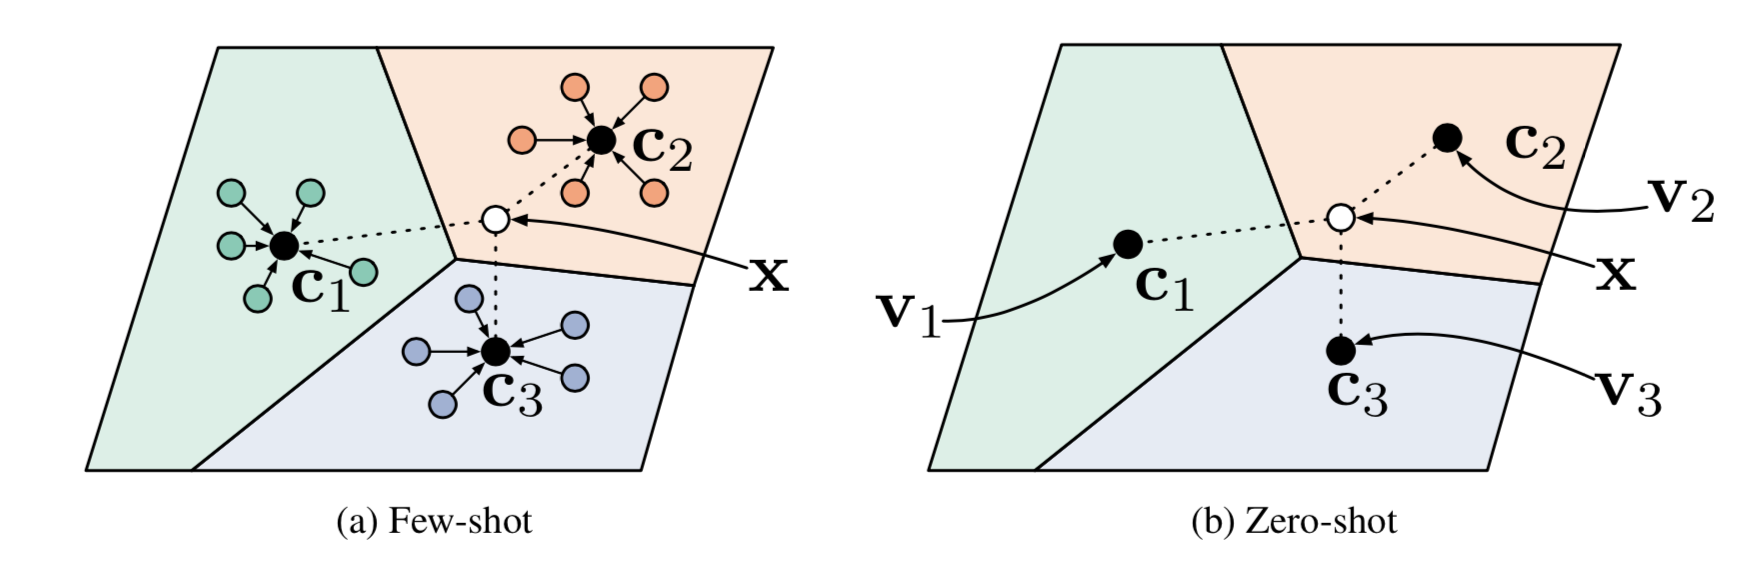
\includegraphics[width=0.60\linewidth]{14_ContinualMetaAndTransferLearning/figures/prototypical_networks.png}
    \caption{Prototypical networks in the few-shot and zero-shot scenarios.}
    \label{fig:my_label}
\end{figure}
The distribution over classes for a given test input $\mathbf{x}$ is a \textit{softmax} over the inverse of distances between the test data embedding and prototype vectors.
\begin{equation}
    P(y=c\vert\mathbf{x})=\text{softmax}(-d_\varphi(f_\theta(\mathbf{x}), \mathbf{v}c)) = \frac{\exp(-d\varphi(f_\theta(\mathbf{x}), \mathbf{v}c))}{\sum{c' \in \mathcal{C}}\exp(-d_\varphi(f_\theta(\mathbf{x}), \mathbf{v}_{c'}))}
\end{equation}
where $d_\varphi$ can be any distance function as long as $\varphi$ is differentiable. In the paper, they used the squared euclidean distance. The loss function is the negative log-likelihood: 
\begin{equation}
    \mathcal{L}(\theta) = -\log P_\theta(y=c\vert\mathbf{x})
\end{equation}

\paragraph{Siamese Neural Networks} are composed of two twin networks and their outputs are jointly trained on top with a function to learn the relationship between pairs of input data samples. The twin networks are identical, sharing the same weights and network parameters. In other words, both refer to the same embedding network that learns an efficient embedding to reveal relationship between pairs of data points.
Convolutional Siamese neural networks have been applied to one-shot image classification\footnote{Koch\&Zemel\&Salakhutdinov, "Siamese Neural Networks for One-shot Image Recognition", 2015}. 
%
\begin{figure}[H]
    \centering
    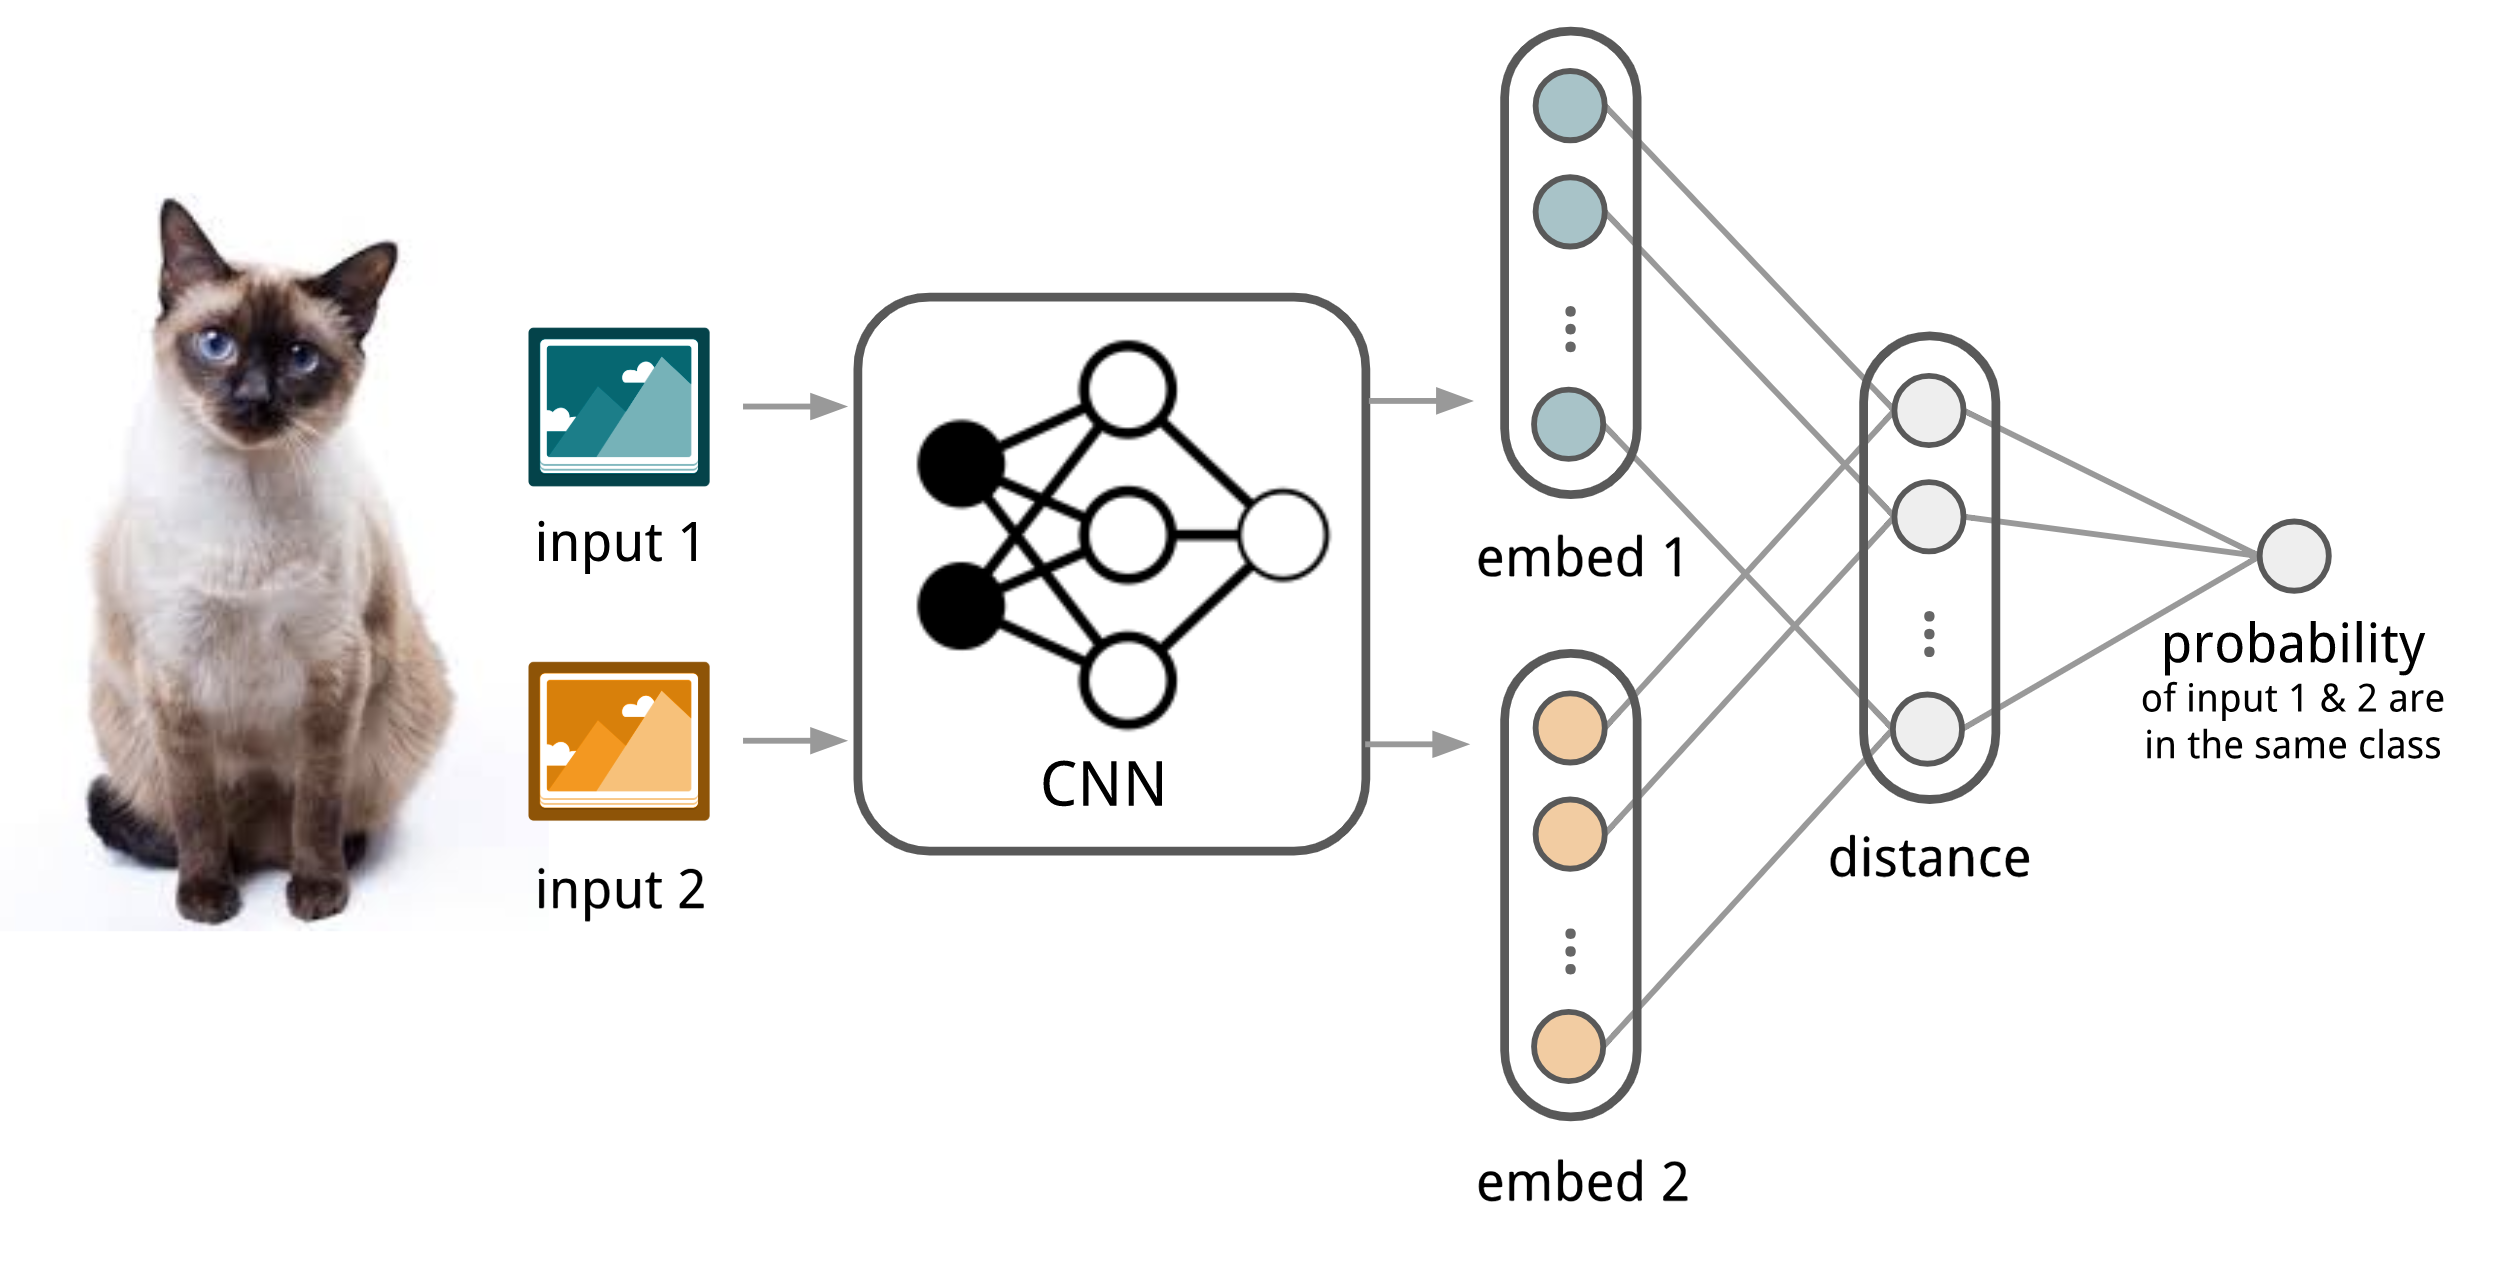
\includegraphics[width=0.99\linewidth]{14_ContinualMetaAndTransferLearning/figures/siamese_convnet.png}
    \caption{The architecture of convolutional siamese neural network for few-show image classification.}
    \label{fig:my_label}
\end{figure}
%
Training: The siamese network is trained for a verification task for telling whether two input images are in the same class. It outputs the probability of two images belonging to the same class.
\begin{enumerate}
    \item First, convolutional siamese network learns to encode two images into feature vectors via a embedding function $f_\theta$ which contains a couple of convolutional layers. 
    \item The L1-distance between two embeddings is $\vert f_\theta(\mathbf{x}i) - f\theta(\mathbf{x}_j) \vert$.
    \item The distance is converted to a probability $p$ by a linear feedforward layer and sigmoid. It is the probability of whether two images are drawn from the same class.
    \item Intuitively the loss is cross entropy because the label is binary. 
    %
    \begin{equation} 
        p(\mathbf{x}_i, \mathbf{x}j) = \sigma(\mathbf{W}\vert f\theta(\mathbf{x}i) - f\theta(\mathbf{x}j) \vert) \\ 
    \end{equation}
    %
    \begin{equation} 
        \mathcal{L}(B) = \sum_{(\mathbf{x}_i, \mathbf{x}j, y_i, y_j)\in B}\mathcal{1}_{y_i=y_j}\log p(\mathbf{x}_i, \mathbf{x}j) + (1-\mathcal{1}_{y_i=y_j})\log (1-p(\mathbf{x}_i, \mathbf{x}_j))
    \end{equation}
    %
\end{enumerate}
Testing: The siamese network processes all the image pairs between a test image and every image in the support set. The final prediction is the class of the support image with the highest probability.
Given a support set $S$ and a test image $\mathbf{x}$, the final predicted class is:
\begin{equation}
   \hat{c}_S(\mathbf{x}) = c(\arg\max{\mathbf{x}_i \in S} P(\mathbf{x}, \mathbf{x}_i)) 
\end{equation}
where $c(\mathbf{x})$ is the class label of an image $\mathbf{x}$ and $\hat{c}(.)$ is the predicted label.




\paragraph{Matching Networks}\footnote{Vinyals et al., "Matching Networks for One Shot Learning", 2016} aim at learning a classifier $c_S$ for any given (small) support set $S=\{x_i, y_i\}_{i=1}^k$ (k-shot classification). This classifier defines a probability distribution over output labels $y$ given a test example $\mathbf{x}$. Similar to other metric-based models, the classifier output is defined as a sum of labels of support samples weighted by attention kernel $a(\mathbf{x}, \mathbf{x}_i)$ - which should be proportional to the similarity between $\mathbf{x}$ and $\mathbf{x}_i$.
%
\begin{figure}[H]
    \centering
    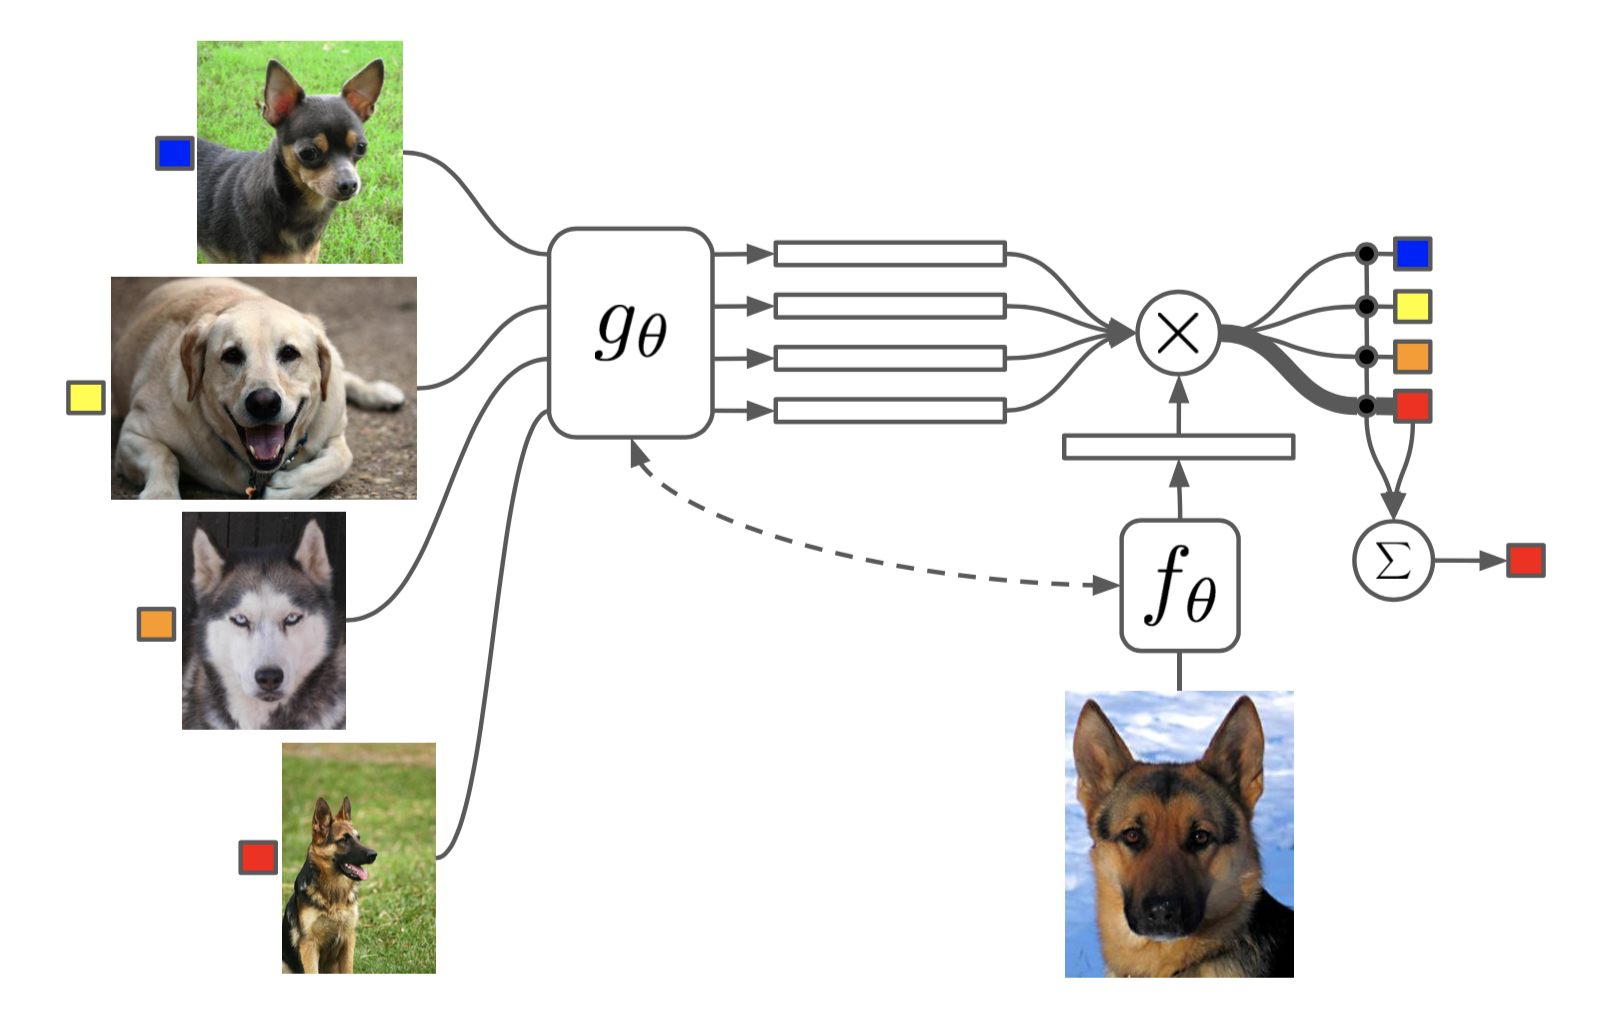
\includegraphics[width=0.80\linewidth]{14_ContinualMetaAndTransferLearning/figures/matching_networks.png}
    \caption{The architecture of Matching Networks}
    \label{fig:my_label}
\end{figure}
%
\begin{equation}
    c_S(\mathbf{x}) = P(y \vert \mathbf{x}, S) = \sum_{i=1}^k a(\mathbf{x}, \mathbf{x}_i) y_i \text{, where }S={(\mathbf{x}i, y_i)}{i=1}^k
\end{equation}
The attention kernel depends on two embedding functions, $f$ and $g$, for encoding the test sample and the support set samples respectively. The attention weight between two data points is the cosine similarity, $\text{cosine}(.)$, between their embedding vectors, normalized by \textit{softmax}:

\begin{equation}
    a(\mathbf{x}, \mathbf{x}_i) = \frac{\exp(\text{cosine}(f(\mathbf{x}), g(\mathbf{x}i))}{\sum{j=1}^k\exp(\text{cosine}(f(\mathbf{x}), g(\mathbf{x}_j))}
\end{equation}

The embedding has to be choosen carefully. In a simple version, an embedding function is a neural network with a single data sample as input. Taking a single data point as input might not be enough to efficiently gauge the entire feature space. Therefore, the Matching Network model further proposed to enhance the embedding functions by taking as input the whole support set $S$ in addition to the original input, so that the learned embedding can be adjusted based on the relationship with other support samples.

\paragraph{Relation Network}\footnote{Sung et al., "Learning to Compare: Relation Network for Few-Shot Learning" 2018} is similar to siamese network but with a few differences:
\begin{itemize}
    \item The relationship is not captured by a simple L1 distance in the feature space, but predicted by a CNN classifier $g_\phi$. The relation score between a pair of inputs, $\mathbf{x}i$ and $\mathbf{x}j$, is $r{i j} = g\phi([\mathbf{x}_i, \mathbf{x}_j])$ where $[.,.]$ is concatenation.
    \item The objective function is MSE loss instead of cross-entropy, because conceptually RN focuses more on predicting relation scores which is more like regression, rather than binary classification, $\mathcal{L}(B) = \sum_{(\mathbf{x}i, \mathbf{x}j, y_i, y_j)\in B} (r{i j} - \mathbf{1}{y_i=y_j})^2$.
\end{itemize}
%
\begin{figure}[H]
    \centering
    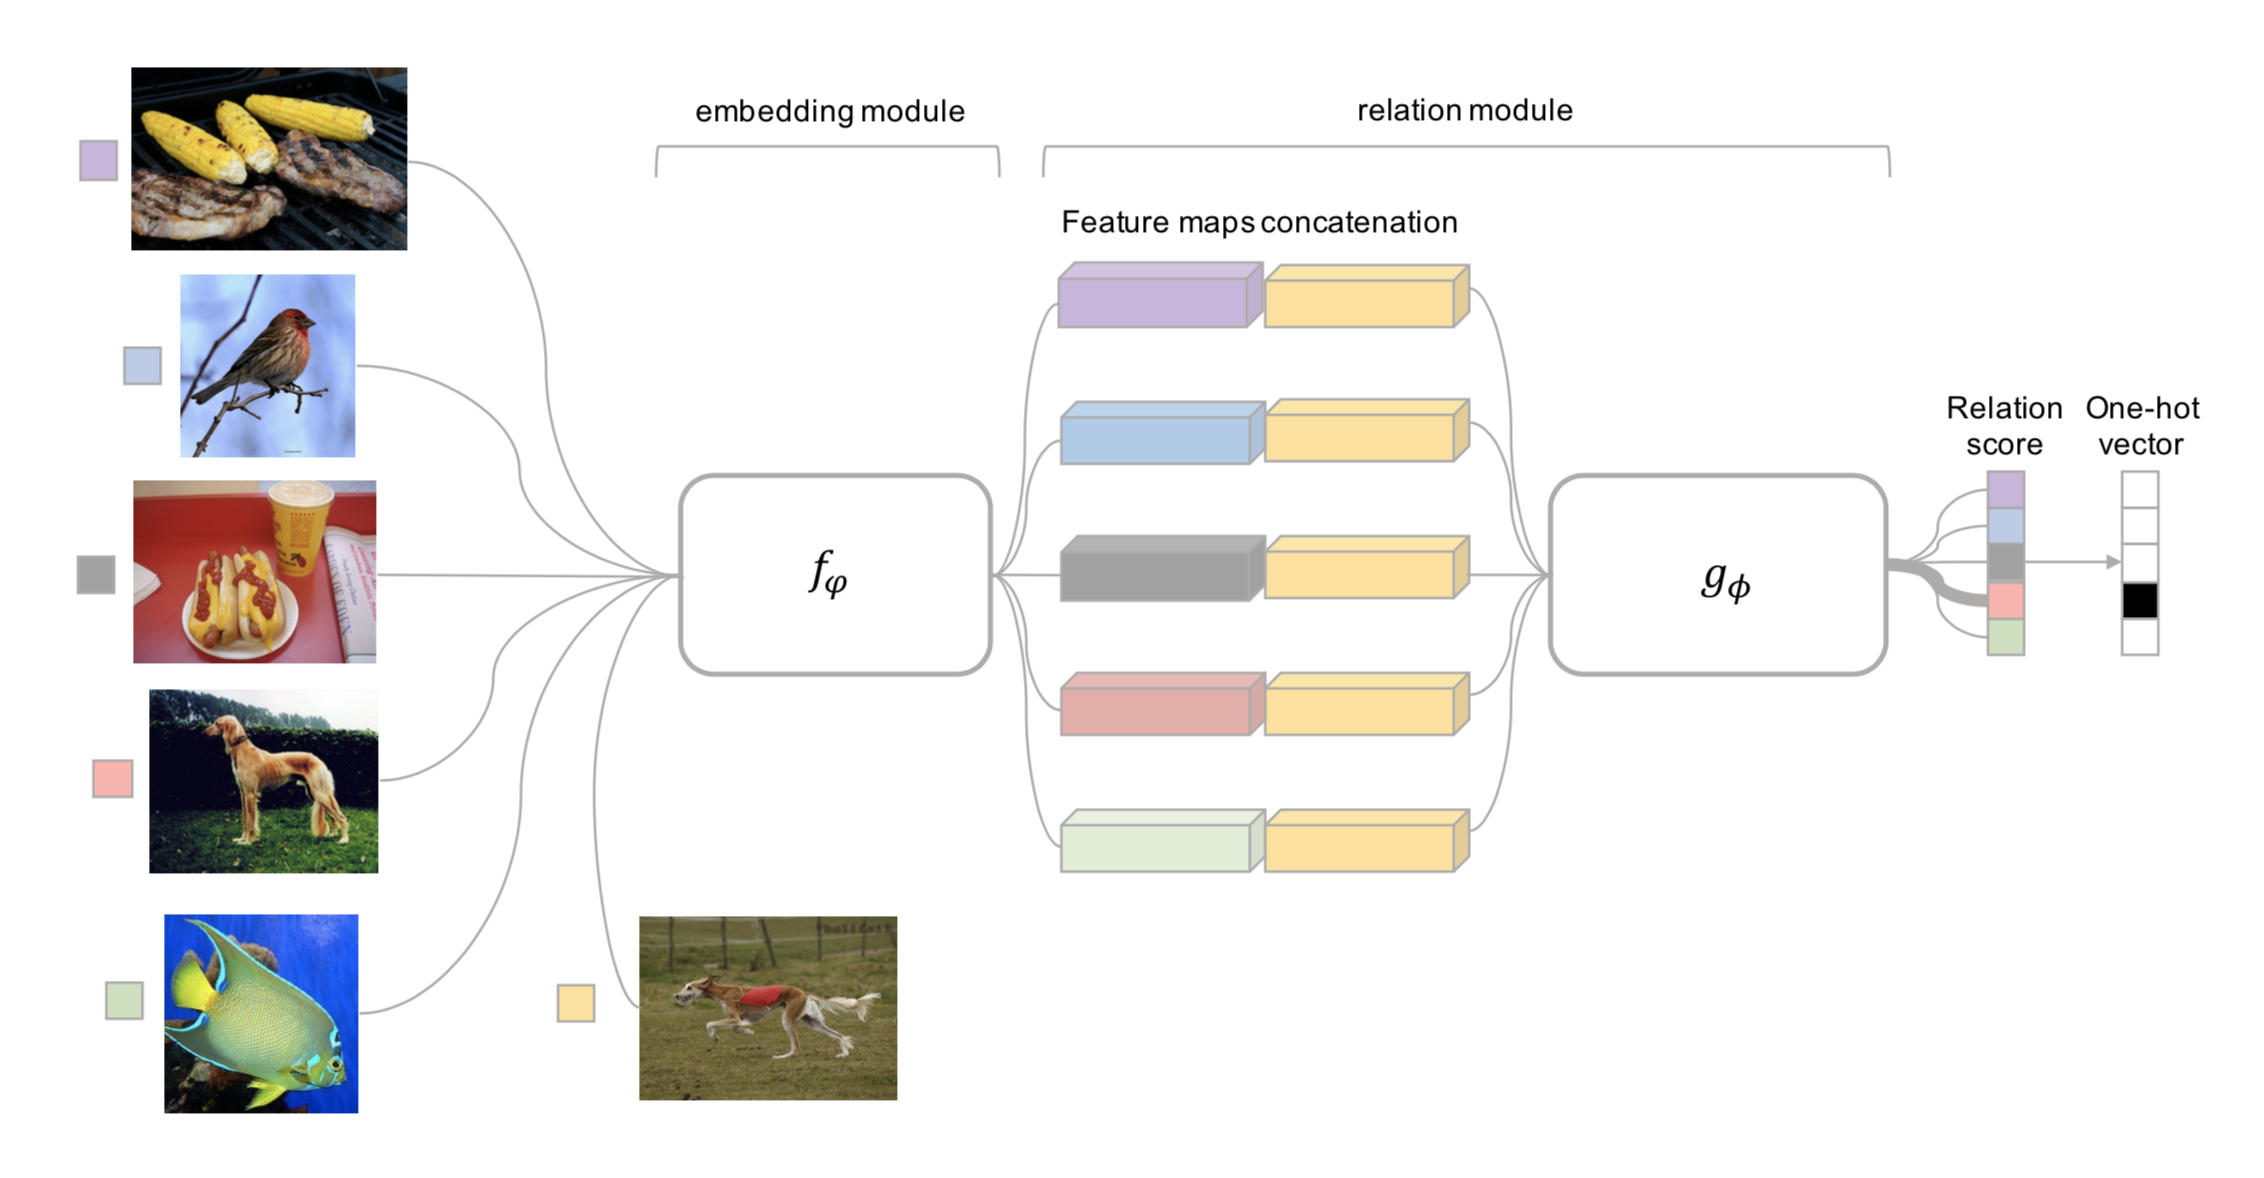
\includegraphics[width=0.95\linewidth]{14_ContinualMetaAndTransferLearning/figures/relation_network.png}
    \caption{Relation Network architecture for a 5-way 1-shot problem with one query example.}
    \label{fig:my_label}
\end{figure}


\subsubsection{Model-based ML}
Model-based meta-learning models make no assumption on the form of $P_{\theta}(y|x)$. Rather it depends on a model designed specifically for fast learning — a model that updates its parameters rapidly with a few training steps. This rapid parameter update can be achieved by its internal architecture or controlled by another meta-learner model.

\paragraph{Hypernetworks}\footnote{Oswald\&Henning\&Sacramento et al., "Continual Learning with Hypernetworks", 2019} are networks that generate
the weights of a target model based on task identity. Continual learning (CL) is less difficult for this class of models thanks to a simple key feature: instead of recalling the input-output relations of all previously seen data, task-conditioned hypernetworks only require rehearsing task-specific weight realizations, which can be maintained in memory using a simple regularizer. Besides achieving state-of-
the-art performance on standard CL benchmarks, additional experiments on long task sequences reveal that task-conditioned hypernetworks display a very large capacity to retain previous memories.
%
\begin{figure}[H]
    \centering
    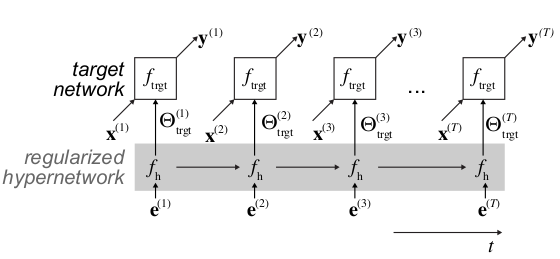
\includegraphics[width=0.85\linewidth]{14_ContinualMetaAndTransferLearning/figures/hypernetwork.png}
    \caption{\textbf{Task-conditioned hypernetworks for continual learning.} Commonly, the parameters of a neural network are directly adjusted from data to solve a task. Here, a weight generator termed hypernetwork is learned instead. Hypernetworks map embedding vectors to weights, which parameterize a target neural network. In a continual learning scenario, a set of task-specific embeddings is learned via backpropagation. Embedding vectors provide task-dependent context and bias the hypernetwork to particular solutions.}
    \label{fig:my_label}
\end{figure}
%
\begin{figure}[H]
    \centering
    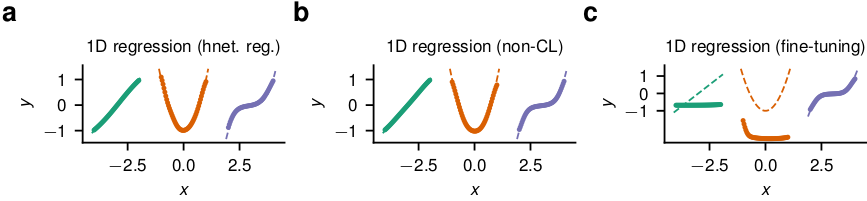
\includegraphics[width=0.95\linewidth]{14_ContinualMetaAndTransferLearning/figures/hypernetwork_toy.png}
    \caption{\textbf{1D nonlinear regression.} \textbf{(a)} Task-conditioned hypernetworks with output regularization can easily model a sequence of polynomials of increasing degree, while learning in a continual fashion. \textbf{(b)} The solution found by a target network which is trained directly on all tasks simultaneously is similar. \textbf{(c)} Fine-tuning, i.e., learning sequentially, leads to forgetting of past tasks. Dashed lines depict ground truth, markers show model predictions.}
    \label{fig:my_label}
\end{figure}
%
\begin{figure}[H]
    \centering
    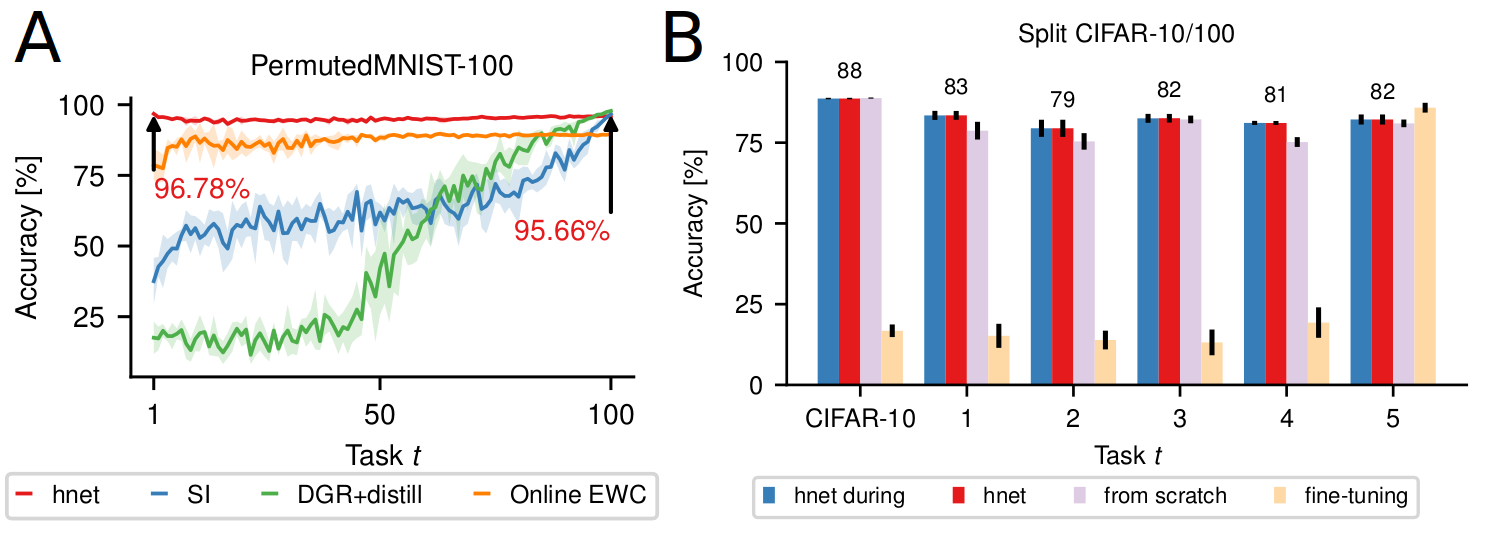
\includegraphics[width=0.95\linewidth]{14_ContinualMetaAndTransferLearning/figures/hypernetwork_results.png}
    \caption{\textbf{Experimental results.} \textbf{(A)} Experiments on the permuted MNIST benchmark.  Final test set classification accuracy on the t-th task after learning one hundred permutations (PermutedMNIST-100). Task-conditioned hypernetworks (hnet, in red) achieve very large memory lifetimes on the permuted MNIST benchmark. Synaptic intelligence (SI, in blue; Zenke et al., 2017), online EWC (in orange; Schwarz et al., 2018) and deep generative replay (DGR+distill, in green; Shin et al., 2017) methods are shown for comparison. \textbf{(B)} Split CIFAR-10/100 continual learning benchmark. Test set accuracies (mean $\pm$ STD, n = 5) on the entire CIFAR-10 dataset and subsequent CIFAR-100 splits. The hypernetwork-protected ResNet-32 displays virtually no forgetting; final averaged performance (hnet, in red) matches the immediate one (hnet-during, in blue). Furthermore, information is transferred across tasks, as performance is higher than when training each task from scratch (purple).}
    \label{fig:my_label}
\end{figure}



\subsubsection{Optimization-Based ML}
Deep learning models learn through backpropagation of gradients. However, the gradient-based optimization is neither designed to cope with a small number of training samples, nor to converge within a small number of optimization steps. Is there a way to adjust the optimization algorithm so that the model can be good at learning with a few examples? This is what optimization-based approach meta-learning algorithms intend for. Look at \textbf{LSTM Meta-Learner}, \textbf{Model-Agnostic Meta-Learning (MAML)} and \textbf{Reptile} for further information (not covered in class). 

\paragraph{Model-Agnostic Meta-Learning (MAML)} is a fairly general optimization algorithm, compatible with any model that learns through gradient descent.
%
Let's say our model is $f_\theta$ with parameters $\theta$. Given a task $\tau_i$ and its associated dataset $(\mathcal{D}^{(i)}\text{train}, \mathcal{D}^{(i)}\text{test})$, we can update the model parameters by one or more gradient descent steps (the following example only contains one step):
%
$$ \theta'i = \theta - \alpha \nabla\theta\mathcal{L}^{(0)}{\tau_i}(f\theta) $$
%
where $\mathcal{L}^{(0)}$ is the loss computed using the mini data batch with id (0).
%
\begin{figure}[H]
    \centering
    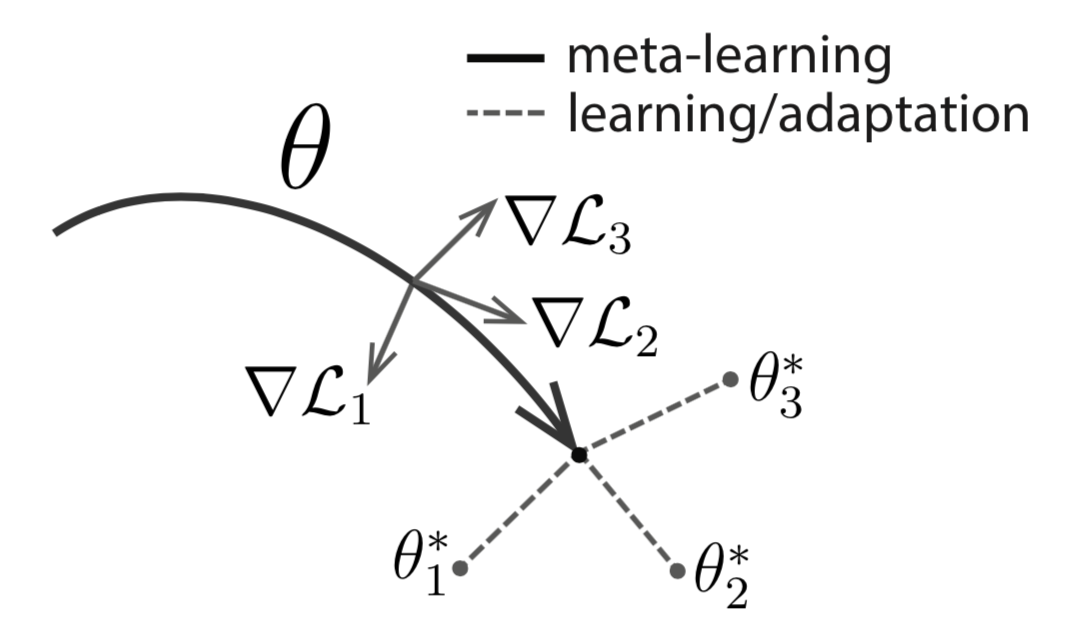
\includegraphics[width=0.5\linewidth]{14_ContinualMetaAndTransferLearning/figures/maml.png}
    \caption{Diagram of MAML.}
    \label{fig:my_label}
\end{figure}
%
The above formula only optimizes for one task. To achieve a good generalization across a variety of tasks, we would like to find the optimal $\theta^*$ so that the task-specific fine-tuning is more efficient. Now, we sample a new data batch with id (1) for updating the meta-objective. The loss, denoted as $\mathcal{L}^{(1)}$, depends on the mini batch (1). The superscripts in $\mathcal{L}^{(0)}$ and $\mathcal{L}^{(1)}$ only indicate different data batches, and they refer to the same loss objective for the same task.
%
\begin{equation}
     \theta^* = \arg\min_\theta \sum_{\tau_i \sim p(\tau)} \mathcal{L}{\tau_i}^{(1)} (f{\theta'i}) = \arg\min\theta \sum_{\tau_i \sim p(\tau)} \mathcal{L}{\tau_i}^{(1)} (f{\theta - \alpha\nabla_\theta \mathcal{L}{\tau_i}^{(0)}(f\theta)})
\end{equation}
%
\begin{equation}
    \theta \leftarrow \theta - \beta \nabla_{\theta} \sum_{\tau_i \sim p(\tau)} \mathcal{L}{\tau_i}^{(1)} (f{\theta - \alpha\nabla_\theta \mathcal{L}{\tau_i}^{(0)}(f\theta)})  \scriptstyle{\text{; updating rule}}
\end{equation}
%

\paragraph{LSTM Meta-Learner}\footnote{Ravi\&Larochelle, "Optimization as a Model for Few-Shot Learning", 2017} is proposed to learn the exact optimization algorithm used to train another learner neural network classifier in the few-shot regime. The parametrization of the model allows it to learn appropriate parameter updates specifically for the scenario where a set amount of updates will be made, while also learning a general initialization of the learner (classifier) network that allows for quick convergence of training.
%
\begin{figure}[H]
    \centering
    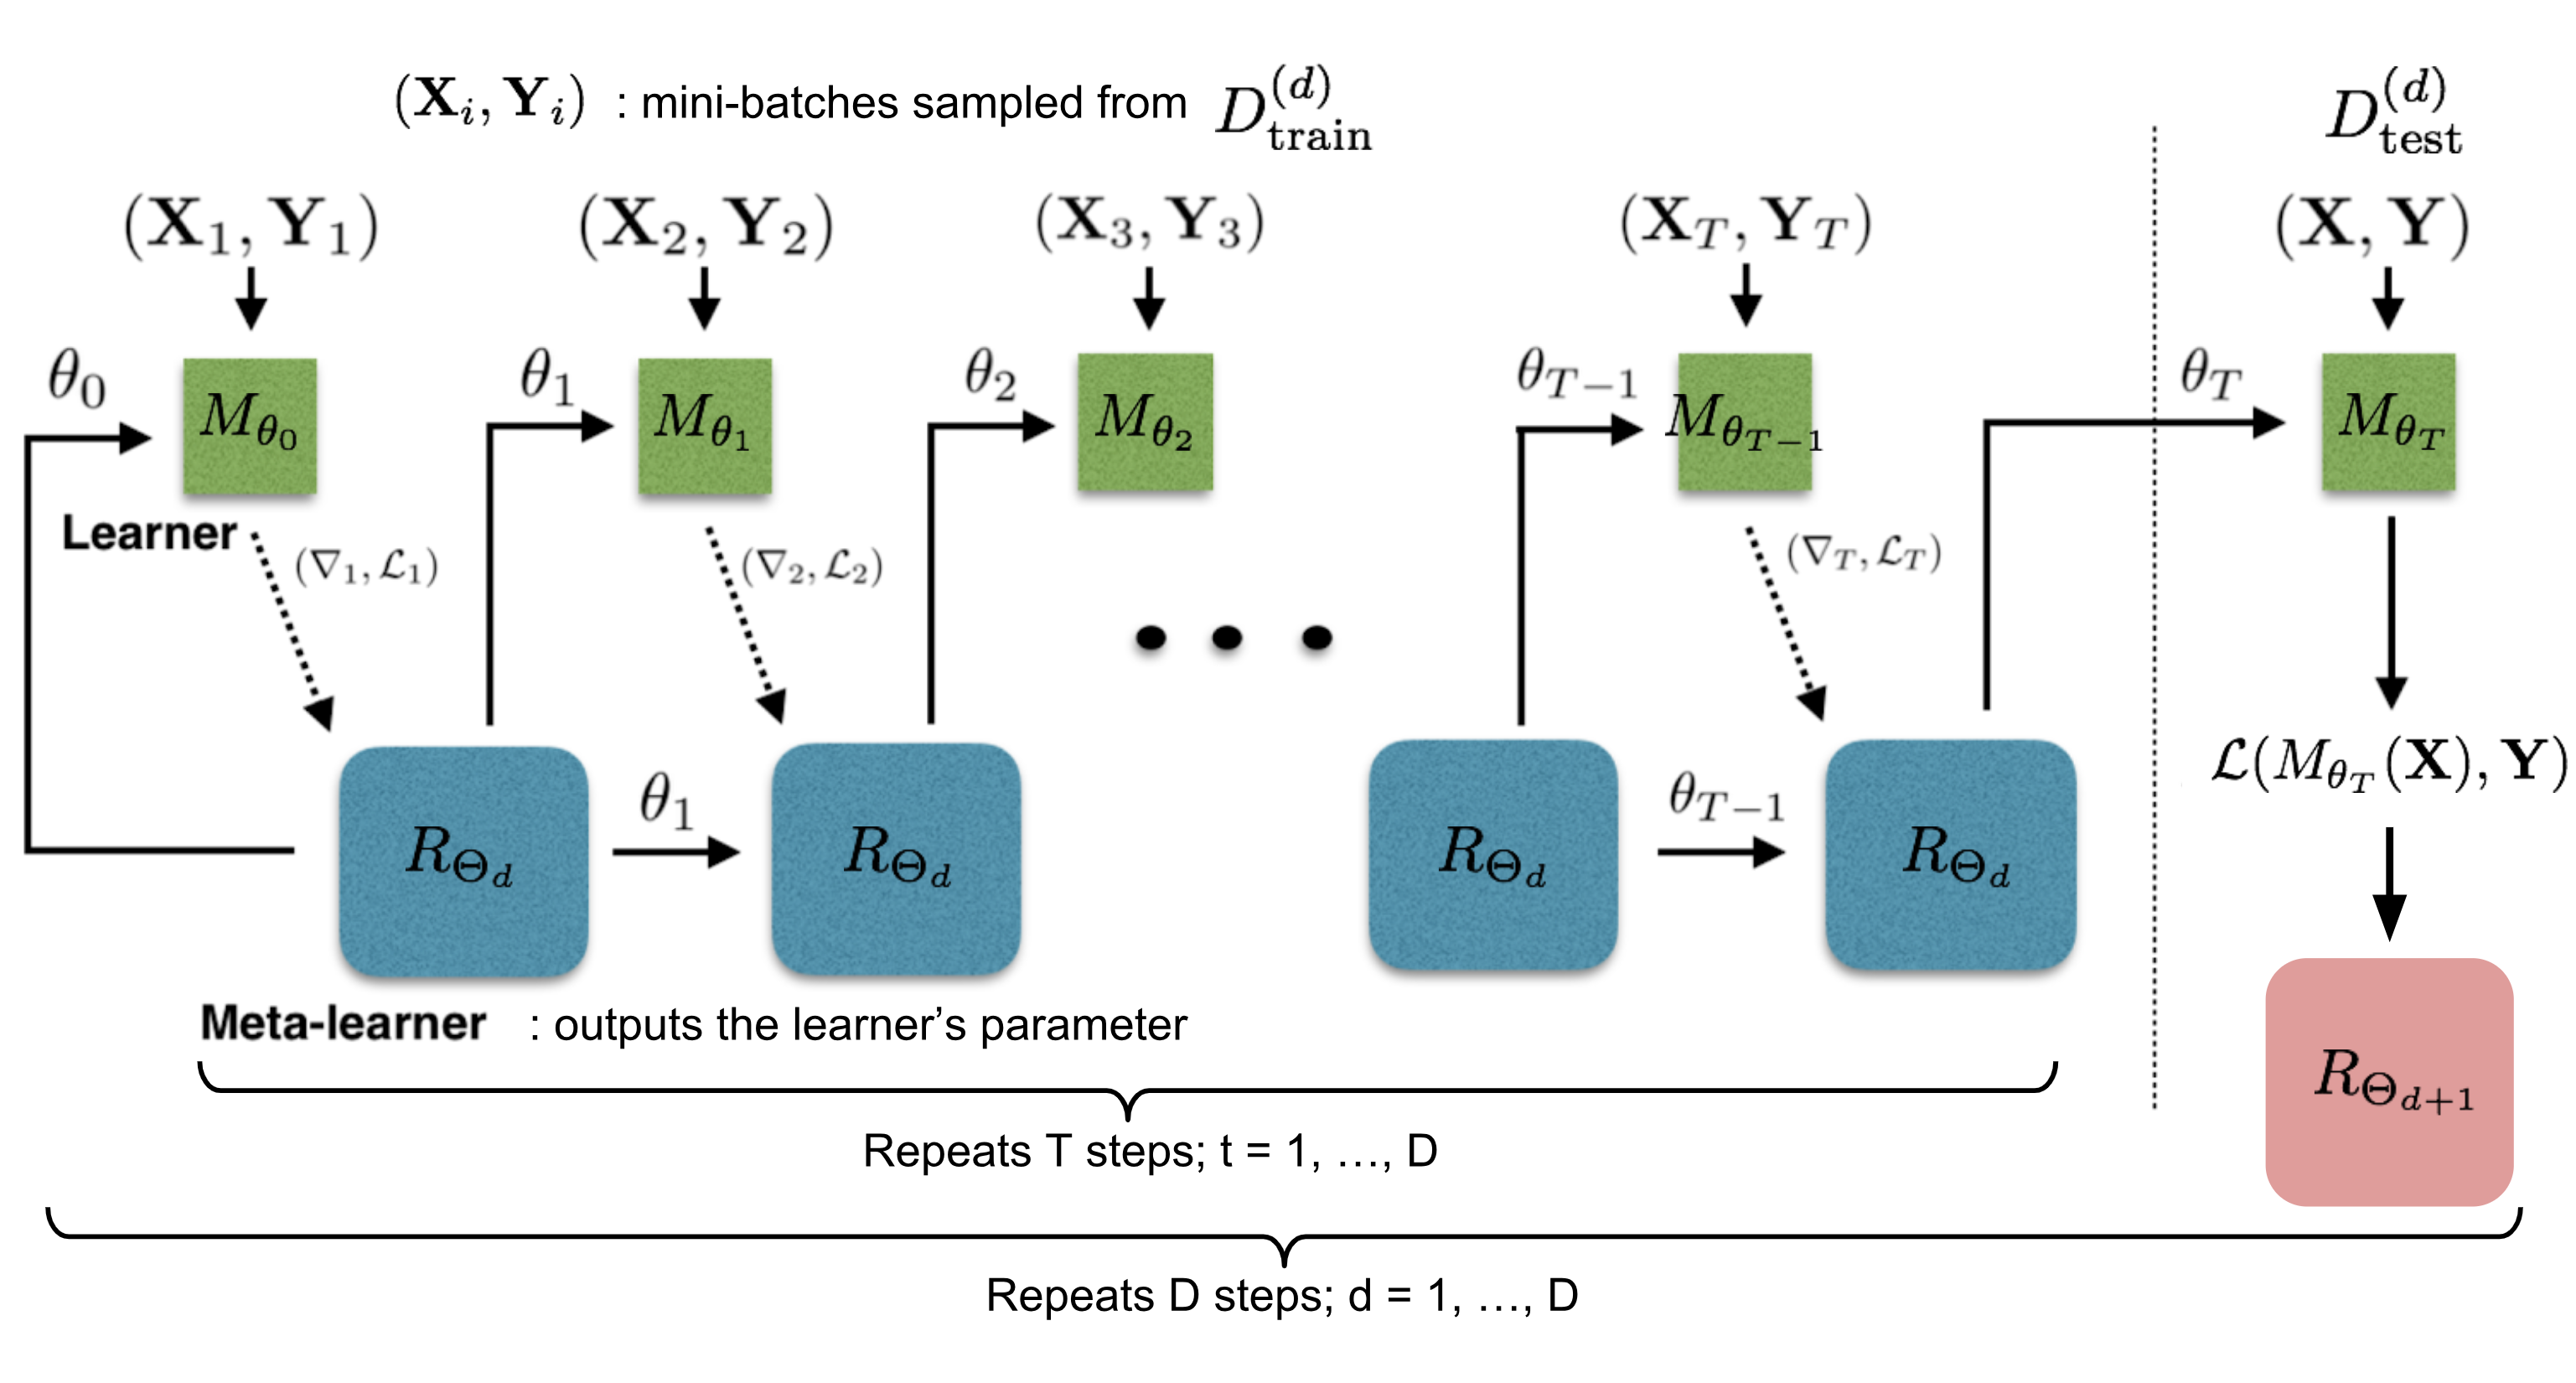
\includegraphics[width=0.8\linewidth]{14_ContinualMetaAndTransferLearning/figures/lstm-meta-learner.png}
    \caption{How the learner $M_\theta$ and the meta-learner $R_\Theta$ are trained. Computational graph for the forward pass of the meta-learner. The dashed line divides examples from the training set $D_{train}$ and test set $D_{test}$.}
    \label{fig:my_label}
\end{figure}



\subsection{Meta-Learning in the Brain}
\hl{...}

\subsubsection{Meta-Learning in the Prefrontal Cortex}
Over the past 20 years, neuroscience research on reward-based learning has converged on a canonical model, under which the neurotransmitter dopamine "stamps in" associations between situations, actions and rewards by modulating the strength of synaptic connections between neurons. However, a growing number of recent findings have placed this standard model under strain. A recent study introduces a new theory, where the dopamine system trains another part of the brain, the prefrontal cortex, to operate as its own free-standing learning system. This new perspective accommodates the findings that motivated the standard model, but also deals with a wider range of observations.
%
\begin{figure}[H]
    \centering
    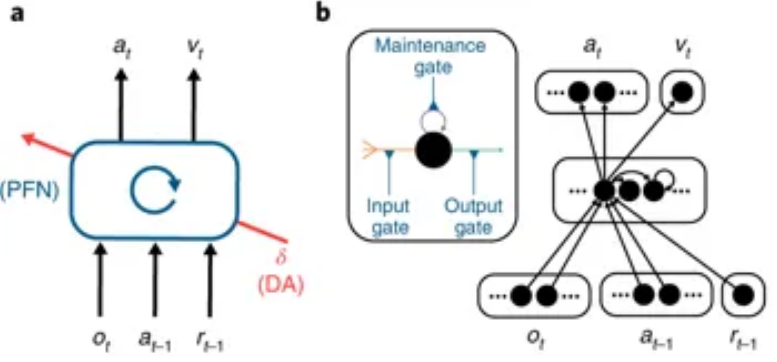
\includegraphics[width=0.8\linewidth]{14_ContinualMetaAndTransferLearning/figures/metalearning_prefrontalcortex.png}
    \caption{\textbf{Meta-RL architecture learns across episodes to learn efficiently within an episode.} \textbf{a} Agent architecture. The prefrontal network (PFN), including sectors of the basal ganglia and the thalamus that connect directly with PFC, is modeled as a recurrent neural network, with synaptic weights adjusted through an RL algorithm driven by dopamine (DA); $o$ is perceptual input, $a$ is action, $r$ is reward, $v$ is state value, $t$ is time-step and $\sigma $ is RPE. The central box denotes a single, fully connected set of LSTM units. \textbf{b} A more detailed schematic of the neural network implementation used in the simulations.}
    \label{fig:sorn}
\end{figure}

\subsubsection{Meta-Learning via Neuromodulation}
Neuromodulators play an important role in meta-learning in the brain. Some of the key modulators are listed below:
Neuromodulatory systems can be seen to mediate the global signals that regulate the distributed learning mechanisms in the brain\footnote{Doya, "Metalearning and neuromodulation", 2002}. Based on the review of experimental data and theoretical models, some key modulators are described below:
\begin{itemize}
    \item[\textbf{Dopamine}] is proposed to act as a "global learning" signal, critical to prediction of rewards and action reinforcement.
    
    \item[\textbf{Serotorin}] is proposed to control the balance between short and long term reward prediction, essentially by variably "discounting" expected future reward sums that may require too much expenditure to achieve.
    
    \item[\textbf{Norepinephrine}] is proposed to facilitate "wide exploration" by stochastic action selection (control exploration vs. exploitation).
    
    \item[\textbf{Acetylcholine}] is proposed to facilitate the balance between memory storage and memory renewal, finding an optimal balance between stability and effectiveness of learning algorithms for the specific environmental task.
\end{itemize}
\begin{figure}[H]
    \centering
    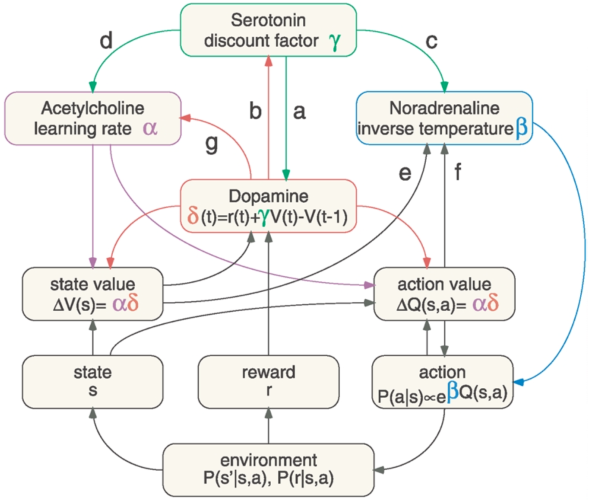
\includegraphics[width=0.8\linewidth]{14_ContinualMetaAndTransferLearning/figures/neuromodulation.png}
    \caption{Computational diagram: Metalearning via neuromodulation.}
    \label{fig:my_label}
\end{figure}


\end{document}